\documentclass[journal]{IEEEtran}

% Shared by main.tex and supplementary.tex

% XeTeX has no Type-1 Times: load the TeX Gyre Termes (Times) files so bold and italic exist
\usepackage{fontspec}
\setmainfont{texgyretermes}[Extension=.otf, UprightFont=*-regular, BoldFont=*-bold,
  ItalicFont=*-italic, BoldItalicFont=*-bolditalic]
\setsansfont{texgyreheros}[Extension=.otf, UprightFont=*-regular, BoldFont=*-bold,
  ItalicFont=*-italic, BoldItalicFont=*-bolditalic]

\usepackage{cite}
\usepackage{amsmath,amssymb,amsfonts}
\usepackage{graphicx}
\usepackage{booktabs}
\usepackage{multirow}
\usepackage{array}
\usepackage{algorithm}
\usepackage{algpseudocode}
\usepackage{xcolor}
\usepackage{tikz}
\usetikzlibrary{arrows.meta,positioning,fit,calc}
\usepackage[hidelinks]{hyperref}

% generated by make_numbers.py from results/puformer_chikusei_x4_v3/paper_analysis/q2n.json
\newcommand{\QtwonVthree}{0.9931}
\newcommand{\QtwonExactUV}{0.9988}
\newcommand{\QtwonExactUVNIR}{0.9998}
\newcommand{\RelErrUV}{0.41}
\newcommand{\RelErrMaxOther}{0.040}
\newcommand{\OracleBicA}{61.6}
\newcommand{\OracleLinA}{57.5}
\newcommand{\OracleModelA}{51.8}
\newcommand{\DefTen}{25\%}
\newcommand{\DefFifty}{75\%}
\newcommand{\CalibPsnrHi}{58.20}
\newcommand{\CalibQHi}{0.9931}
\newcommand{\CalibPsnrMid}{52.15}
\newcommand{\CalibQMid}{0.9904}

% generated by make_tables.py - do not edit
\makeatletter
\@namedef{pav@S-PSNR}{50.63}
\@namedef{pav@S-PSNR_psrt}{50.22}
\@namedef{pav@S-MPSNR_peak1}{51.11}
\@namedef{pav@S-SSIM}{0.9970}
\@namedef{pav@S-SSIM_psrt}{0.9974}
\@namedef{pav@S-SAM}{1.895}
\@namedef{pav@S-ERGAS}{0.621}
\@namedef{pav@S-RMSE_DN}{23.7}
\@namedef{pav@S-CC}{0.9994}
\@namedef{pav@S-SCC}{0.9995}
\@namedef{pav@S-Q2n}{0.9751}
\@namedef{pav@E-PSNR}{50.69}
\@namedef{pav@E-PSNR_psrt}{50.28}
\@namedef{pav@E-MPSNR_peak1}{51.17}
\@namedef{pav@E-SSIM}{0.9970}
\@namedef{pav@E-SSIM_psrt}{0.9974}
\@namedef{pav@E-SAM}{1.883}
\@namedef{pav@E-ERGAS}{0.617}
\@namedef{pav@E-RMSE_DN}{23.5}
\@namedef{pav@E-CC}{0.9994}
\@namedef{pav@E-SCC}{0.9995}
\@namedef{pav@E-Q2n}{0.9753}
\@namedef{pav@rank-PSNR}{1}
\@namedef{pav@tipbest-PSNR}{47.1597}
\@namedef{pav@tipbestname-PSNR}{Two-stage diffusion}
\@namedef{pav@rank-SSIM}{1}
\@namedef{pav@tipbest-SSIM}{0.9972}
\@namedef{pav@tipbestname-SSIM}{SMGU}
\@namedef{pav@rank-SAM}{13}
\@namedef{pav@tipbest-SAM}{1.4542}
\@namedef{pav@tipbestname-SAM}{Two-stage diffusion}
\@namedef{pav@rank-ERGAS}{1}
\@namedef{pav@tipbest-ERGAS}{0.8262}
\@namedef{pav@tipbestname-ERGAS}{Two-stage diffusion}
\@namedef{pav@rank-Q2n}{16}
\@namedef{pav@tipbest-Q2n}{0.9987}
\@namedef{pav@tipbestname-Q2n}{OTPNet}
\@namedef{pav@rank-CC}{1}
\@namedef{pav@tipbest-CC}{0.9985}
\@namedef{pav@tipbestname-CC}{Two-stage diffusion}
\@namedef{pav@rank-SCC}{1}
\@namedef{pav@tipbest-SCC}{0.9976}
\@namedef{pav@tipbestname-SCC}{Two-stage diffusion}
\@namedef{pav@rank-RMSE_DN}{1}
\@namedef{pav@tipbest-RMSE_DN}{35.71}
\@namedef{pav@tipbestname-RMSE_DN}{Two-stage diffusion}
\@namedef{pav@first}{6}
\@namedef{pav@firstlist}{PSNR, SSIM, ERGAS, CC, SCC, RMSE_DN}
\@namedef{pav@gain-PSNR}{3.53}
\@namedef{pav@red-RMSE_DN}{34.1}
\@namedef{pav@red-ERGAS}{25.3}
\@namedef{pav@red-SAM}{-29.5}
\@namedef{pav@cons-H}{79.9}
\@namedef{pav@cons-M}{77.6}
\@namedef{pav@gsa-PSNR}{34.78}
\@namedef{pav@gsa-SAM}{5.23}
\@namedef{pav@tipgsa-PSNR}{35.35}
\@namedef{pav@gsa-gap}{0.57}
\@namedef{pav@bic-PSNR}{25.52}
\@namedef{pav@iters}{93{,}850}
\@namedef{pav@hours}{10.2}
\@namedef{pav@params}{9.99}
\@namedef{pav@patches}{1.50}
\@namedef{pav@best-it}{43{,}000}
\@namedef{pav@best-val}{48.58}
\@namedef{pav@test-peak}{50.66}
\@namedef{pav@test-peak-it}{25{,}000}
\@namedef{pav@test-at-best}{50.63}
\@namedef{pav@test-end}{50.58}
\@namedef{pav@infer}{0.18}
\@namedef{pav@visual-tile}{3}
\@namedef{pav@blur-fixed-loss-min}{3.3}
\@namedef{pav@blur-fixed-loss-max}{6.8}
\@namedef{pav@blur-swap-loss-max}{0.11}
\@namedef{pav@srf-swap-delta}{-0.2}
\@namedef{pav@noise40-margin}{12.8}
\@namedef{pav@noise35-margin}{9.8}
\@namedef{pav@noise30-margin}{6.0}
\@namedef{pav@q2n}{0.9753}
\@namedef{pav@q2n-def10}{96\%}
\@namedef{pav@q2n-def50}{99\%}
\@namedef{pav@q2n-relmax}{0.561}
\@namedef{pav@q2n-relmin}{0.256}
\@namedef{pav@calib-psnr-hi}{50.69}
\@namedef{pav@calib-q-hi}{0.9753}
\@namedef{pav@calib-psnr-mid}{44.32}
\@namedef{pav@calib-q-mid}{0.9724}
\@namedef{pav@water-1}{11}
\@namedef{pav@water-2}{63}
\@namedef{pav@water-3}{7}
\@namedef{pav@water-4}{13}
\@namedef{pav@sam-water}{2.95}
\@namedef{pav@sam-nowater}{1.56}
\@namedef{pav@sam-nowater-2}{1.41}
\@namedef{pav@sam-dark10}{34}
\@namedef{pav@gsa-sam-water}{6.98}
\@namedef{pav@gsa-sam-nowater}{4.70}
\@namedef{pav@gsa-sam-nowater-2}{3.62}
\@namedef{pav@gsa-sam-dark10}{27}
\@namedef{pav@noise-floor}{1.01}
\@namedef{pav@noise-floor-2}{1.65}
\@namedef{pav@noise-floor-dark}{3.8}
\@namedef{pav@noise-floor-bright}{0.23}
\@namedef{pav@zero-pixels}{0}
\makeatother

% \pav{key}: a value generated by make_tables.py from the Pavia Centre result files
\newcommand{\pav}[1]{\ifcsname pav@#1\endcsname\csname pav@#1\endcsname\else\textbf{??#1??}\fi}
% \qone{key}: a value generated by make_q1_tables.py from results/q1 (equal-budget benchmark, ablations)
\IfFileExists{tables/q1_numbers.tex}{% generated by make_q1_tables.py - do not edit
\expandafter\def\csname qone@abl-conv-absdelta\endcsname{0.02}
\expandafter\def\csname qone@abl-conv-consH\endcsname{78.5}
\expandafter\def\csname qone@abl-conv-consM\endcsname{73.9}
\expandafter\def\csname qone@abl-conv-delta\endcsname{-0.02}
\expandafter\def\csname qone@abl-conv-params\endcsname{9.94}
\expandafter\def\csname qone@abl-conv-psnr\endcsname{50.60}
\expandafter\def\csname qone@abl-conv-row\endcsname{j}
\expandafter\def\csname qone@abl-conv-sam\endcsname{1.909}
\expandafter\def\csname qone@abl-full-consH\endcsname{77.6}
\expandafter\def\csname qone@abl-full-consM\endcsname{74.8}
\expandafter\def\csname qone@abl-full-fixed\endcsname{43.13}
\expandafter\def\csname qone@abl-full-fixedloss\endcsname{7.50}
\expandafter\def\csname qone@abl-full-mean\endcsname{50.62}
\expandafter\def\csname qone@abl-full-nseeds\endcsname{3}
\expandafter\def\csname qone@abl-full-params\endcsname{9.99}
\expandafter\def\csname qone@abl-full-psnr\endcsname{50.63}
\expandafter\def\csname qone@abl-full-row\endcsname{a}
\expandafter\def\csname qone@abl-full-sam\endcsname{1.897}
\expandafter\def\csname qone@abl-full-std\endcsname{0.02}
\expandafter\def\csname qone@abl-full-swap\endcsname{50.50}
\expandafter\def\csname qone@abl-full-swaploss\endcsname{0.13}
\expandafter\def\csname qone@abl-k1-absdelta\endcsname{0.02}
\expandafter\def\csname qone@abl-k1-consH\endcsname{71.3}
\expandafter\def\csname qone@abl-k1-consM\endcsname{70.8}
\expandafter\def\csname qone@abl-k1-delta\endcsname{-0.02}
\expandafter\def\csname qone@abl-k1-params\endcsname{3.33}
\expandafter\def\csname qone@abl-k1-psnr\endcsname{50.60}
\expandafter\def\csname qone@abl-k1-row\endcsname{g}
\expandafter\def\csname qone@abl-k1-sam\endcsname{1.909}
\expandafter\def\csname qone@abl-k2-absdelta\endcsname{0.02}
\expandafter\def\csname qone@abl-k2-consH\endcsname{75.0}
\expandafter\def\csname qone@abl-k2-consM\endcsname{73.4}
\expandafter\def\csname qone@abl-k2-delta\endcsname{+0.02}
\expandafter\def\csname qone@abl-k2-params\endcsname{6.66}
\expandafter\def\csname qone@abl-k2-psnr\endcsname{50.64}
\expandafter\def\csname qone@abl-k2-row\endcsname{h}
\expandafter\def\csname qone@abl-k2-sam\endcsname{1.901}
\expandafter\def\csname qone@abl-k4-absdelta\endcsname{0.06}
\expandafter\def\csname qone@abl-k4-consH\endcsname{80.2}
\expandafter\def\csname qone@abl-k4-consM\endcsname{76.3}
\expandafter\def\csname qone@abl-k4-delta\endcsname{+0.06}
\expandafter\def\csname qone@abl-k4-params\endcsname{13.32}
\expandafter\def\csname qone@abl-k4-psnr\endcsname{50.68}
\expandafter\def\csname qone@abl-k4-row\endcsname{i}
\expandafter\def\csname qone@abl-k4-sam\endcsname{1.894}
\expandafter\def\csname qone@abl-l1-absdelta\endcsname{0.03}
\expandafter\def\csname qone@abl-l1-consH\endcsname{77.5}
\expandafter\def\csname qone@abl-l1-consM\endcsname{75.7}
\expandafter\def\csname qone@abl-l1-delta\endcsname{+0.03}
\expandafter\def\csname qone@abl-l1-params\endcsname{9.99}
\expandafter\def\csname qone@abl-l1-psnr\endcsname{50.66}
\expandafter\def\csname qone@abl-l1-row\endcsname{l}
\expandafter\def\csname qone@abl-l1-sam\endcsname{1.897}
\expandafter\def\csname qone@abl-learned-absdelta\endcsname{0.06}
\expandafter\def\csname qone@abl-learned-consH\endcsname{73.6}
\expandafter\def\csname qone@abl-learned-consM\endcsname{72.6}
\expandafter\def\csname qone@abl-learned-delta\endcsname{-0.06}
\expandafter\def\csname qone@abl-learned-fixed\endcsname{49.33}
\expandafter\def\csname qone@abl-learned-fixedloss\endcsname{1.24}
\expandafter\def\csname qone@abl-learned-params\endcsname{9.99}
\expandafter\def\csname qone@abl-learned-psnr\endcsname{50.57}
\expandafter\def\csname qone@abl-learned-row\endcsname{e}
\expandafter\def\csname qone@abl-learned-sam\endcsname{1.908}
\expandafter\def\csname qone@abl-nodeep-absdelta\endcsname{0.12}
\expandafter\def\csname qone@abl-nodeep-consH\endcsname{77.7}
\expandafter\def\csname qone@abl-nodeep-consM\endcsname{74.6}
\expandafter\def\csname qone@abl-nodeep-delta\endcsname{-0.12}
\expandafter\def\csname qone@abl-nodeep-params\endcsname{9.99}
\expandafter\def\csname qone@abl-nodeep-psnr\endcsname{50.50}
\expandafter\def\csname qone@abl-nodeep-row\endcsname{m}
\expandafter\def\csname qone@abl-nodeep-sam\endcsname{1.900}
\expandafter\def\csname qone@abl-nomem-absdelta\endcsname{0.05}
\expandafter\def\csname qone@abl-nomem-consH\endcsname{77.2}
\expandafter\def\csname qone@abl-nomem-consM\endcsname{74.8}
\expandafter\def\csname qone@abl-nomem-delta\endcsname{+0.05}
\expandafter\def\csname qone@abl-nomem-params\endcsname{9.98}
\expandafter\def\csname qone@abl-nomem-psnr\endcsname{50.67}
\expandafter\def\csname qone@abl-nomem-row\endcsname{f}
\expandafter\def\csname qone@abl-nomem-sam\endcsname{1.898}
\expandafter\def\csname qone@abl-nophys-absdelta\endcsname{0.17}
\expandafter\def\csname qone@abl-nophys-consH\endcsname{68.9}
\expandafter\def\csname qone@abl-nophys-consM\endcsname{73.3}
\expandafter\def\csname qone@abl-nophys-delta\endcsname{-0.17}
\expandafter\def\csname qone@abl-nophys-params\endcsname{9.99}
\expandafter\def\csname qone@abl-nophys-psnr\endcsname{50.46}
\expandafter\def\csname qone@abl-nophys-row\endcsname{b}
\expandafter\def\csname qone@abl-nophys-sam\endcsname{1.928}
\expandafter\def\csname qone@abl-nores-absdelta\endcsname{0.01}
\expandafter\def\csname qone@abl-nores-consH\endcsname{75.7}
\expandafter\def\csname qone@abl-nores-consM\endcsname{73.8}
\expandafter\def\csname qone@abl-nores-delta\endcsname{-0.01}
\expandafter\def\csname qone@abl-nores-params\endcsname{9.99}
\expandafter\def\csname qone@abl-nores-psnr\endcsname{50.62}
\expandafter\def\csname qone@abl-nores-row\endcsname{c}
\expandafter\def\csname qone@abl-nores-sam\endcsname{1.900}
\expandafter\def\csname qone@abl-seed-gain\endcsname{0.08}
\expandafter\def\csname qone@abl-window-absdelta\endcsname{0.01}
\expandafter\def\csname qone@abl-window-consH\endcsname{78.6}
\expandafter\def\csname qone@abl-window-consM\endcsname{75.5}
\expandafter\def\csname qone@abl-window-delta\endcsname{+0.01}
\expandafter\def\csname qone@abl-window-params\endcsname{9.99}
\expandafter\def\csname qone@abl-window-psnr\endcsname{50.63}
\expandafter\def\csname qone@abl-window-row\endcsname{k}
\expandafter\def\csname qone@abl-window-sam\endcsname{1.898}
\expandafter\def\csname qone@abl-zeros-absdelta\endcsname{0.08}
\expandafter\def\csname qone@abl-zeros-consH\endcsname{74.5}
\expandafter\def\csname qone@abl-zeros-consM\endcsname{73.0}
\expandafter\def\csname qone@abl-zeros-delta\endcsname{-0.08}
\expandafter\def\csname qone@abl-zeros-fixed\endcsname{46.55}
\expandafter\def\csname qone@abl-zeros-fixedloss\endcsname{3.97}
\expandafter\def\csname qone@abl-zeros-mean\endcsname{50.54}
\expandafter\def\csname qone@abl-zeros-nseeds\endcsname{3}
\expandafter\def\csname qone@abl-zeros-params\endcsname{9.99}
\expandafter\def\csname qone@abl-zeros-psnr\endcsname{50.52}
\expandafter\def\csname qone@abl-zeros-row\endcsname{d}
\expandafter\def\csname qone@abl-zeros-sam\endcsname{1.915}
\expandafter\def\csname qone@abl-zeros-std\endcsname{0.03}
\expandafter\def\csname qone@abl-zeros-swap\endcsname{49.64}
\expandafter\def\csname qone@abl-zeros-swaploss\endcsname{0.88}
\expandafter\def\csname qone@altloss-max\endcsname{3.4}
\expandafter\def\csname qone@altloss-min\endcsname{0.9}
\expandafter\def\csname qone@blind-chikusei-grid\endcsname{0.05}
\expandafter\def\csname qone@blind-chikusei-max-sigerr\endcsname{0.000}
\expandafter\def\csname qone@blind-chikusei-noisy-nominal-exact_fixed\endcsname{49.28}
\expandafter\def\csname qone@blind-chikusei-noisy-nominal-learned_fixed\endcsname{49.37}
\expandafter\def\csname qone@blind-chikusei-noisy-nominal-zeros_fixed\endcsname{49.50}
\expandafter\def\csname qone@blind-chikusei-noisy-worst-exact_estimated\endcsname{49.28}
\expandafter\def\csname qone@blind-chikusei-noisy-worst-exact_fixed\endcsname{47.58}
\expandafter\def\csname qone@blind-chikusei-noisy-worst-learned_fixed\endcsname{48.66}
\expandafter\def\csname qone@blind-chikusei-noisy-worst-zeros_estimated\endcsname{48.80}
\expandafter\def\csname qone@blind-chikusei-nominal-exact_fixed\endcsname{57.95}
\expandafter\def\csname qone@blind-chikusei-nominal-learned_fixed\endcsname{57.73}
\expandafter\def\csname qone@blind-chikusei-nominal-zeros_fixed\endcsname{57.79}
\expandafter\def\csname qone@blind-chikusei-s1.5-exact_estimated\endcsname{57.75}
\expandafter\def\csname qone@blind-chikusei-s1.5-exact_fixed\endcsname{51.41}
\expandafter\def\csname qone@blind-chikusei-s1.5-exact_oracle\endcsname{57.75}
\expandafter\def\csname qone@blind-chikusei-s1.5-learned_fixed\endcsname{54.28}
\expandafter\def\csname qone@blind-chikusei-s1.5-noise-exact_estimated\endcsname{49.38}
\expandafter\def\csname qone@blind-chikusei-s1.5-noise-exact_fixed\endcsname{47.58}
\expandafter\def\csname qone@blind-chikusei-s1.5-noise-exact_oracle\endcsname{49.38}
\expandafter\def\csname qone@blind-chikusei-s1.5-noise-learned_fixed\endcsname{48.66}
\expandafter\def\csname qone@blind-chikusei-s1.5-noise-sigerr\endcsname{0.000}
\expandafter\def\csname qone@blind-chikusei-s1.5-noise-zeros_estimated\endcsname{48.80}
\expandafter\def\csname qone@blind-chikusei-s1.5-sigerr\endcsname{0.000}
\expandafter\def\csname qone@blind-chikusei-s1.5-zeros_estimated\endcsname{54.39}
\expandafter\def\csname qone@blind-chikusei-s2-exact_estimated\endcsname{57.95}
\expandafter\def\csname qone@blind-chikusei-s2-exact_fixed\endcsname{57.95}
\expandafter\def\csname qone@blind-chikusei-s2-exact_oracle\endcsname{57.95}
\expandafter\def\csname qone@blind-chikusei-s2-learned_fixed\endcsname{57.73}
\expandafter\def\csname qone@blind-chikusei-s2-noise-exact_estimated\endcsname{49.28}
\expandafter\def\csname qone@blind-chikusei-s2-noise-exact_fixed\endcsname{49.28}
\expandafter\def\csname qone@blind-chikusei-s2-noise-exact_oracle\endcsname{49.28}
\expandafter\def\csname qone@blind-chikusei-s2-noise-learned_fixed\endcsname{49.37}
\expandafter\def\csname qone@blind-chikusei-s2-noise-sigerr\endcsname{0.000}
\expandafter\def\csname qone@blind-chikusei-s2-noise-zeros_estimated\endcsname{49.50}
\expandafter\def\csname qone@blind-chikusei-s2-sigerr\endcsname{0.000}
\expandafter\def\csname qone@blind-chikusei-s2-zeros_estimated\endcsname{57.79}
\expandafter\def\csname qone@blind-chikusei-s2.5-exact_estimated\endcsname{57.86}
\expandafter\def\csname qone@blind-chikusei-s2.5-exact_fixed\endcsname{54.59}
\expandafter\def\csname qone@blind-chikusei-s2.5-exact_oracle\endcsname{57.86}
\expandafter\def\csname qone@blind-chikusei-s2.5-learned_fixed\endcsname{56.19}
\expandafter\def\csname qone@blind-chikusei-s2.5-noise-exact_estimated\endcsname{49.36}
\expandafter\def\csname qone@blind-chikusei-s2.5-noise-exact_fixed\endcsname{48.66}
\expandafter\def\csname qone@blind-chikusei-s2.5-noise-exact_oracle\endcsname{49.36}
\expandafter\def\csname qone@blind-chikusei-s2.5-noise-learned_fixed\endcsname{49.11}
\expandafter\def\csname qone@blind-chikusei-s2.5-noise-sigerr\endcsname{0.000}
\expandafter\def\csname qone@blind-chikusei-s2.5-noise-zeros_estimated\endcsname{49.41}
\expandafter\def\csname qone@blind-chikusei-s2.5-sigerr\endcsname{0.000}
\expandafter\def\csname qone@blind-chikusei-s2.5-zeros_estimated\endcsname{56.62}
\expandafter\def\csname qone@blind-chikusei-s3-exact_estimated\endcsname{57.70}
\expandafter\def\csname qone@blind-chikusei-s3-exact_fixed\endcsname{52.32}
\expandafter\def\csname qone@blind-chikusei-s3-exact_oracle\endcsname{57.70}
\expandafter\def\csname qone@blind-chikusei-s3-learned_fixed\endcsname{54.72}
\expandafter\def\csname qone@blind-chikusei-s3-noise-exact_estimated\endcsname{49.40}
\expandafter\def\csname qone@blind-chikusei-s3-noise-exact_fixed\endcsname{47.94}
\expandafter\def\csname qone@blind-chikusei-s3-noise-exact_oracle\endcsname{49.40}
\expandafter\def\csname qone@blind-chikusei-s3-noise-learned_fixed\endcsname{48.77}
\expandafter\def\csname qone@blind-chikusei-s3-noise-sigerr\endcsname{0.000}
\expandafter\def\csname qone@blind-chikusei-s3-noise-zeros_estimated\endcsname{49.20}
\expandafter\def\csname qone@blind-chikusei-s3-sigerr\endcsname{0.000}
\expandafter\def\csname qone@blind-chikusei-s3-zeros_estimated\endcsname{55.36}
\expandafter\def\csname qone@blind-chikusei-worst-exact_estimated\endcsname{57.70}
\expandafter\def\csname qone@blind-chikusei-worst-exact_fixed\endcsname{51.41}
\expandafter\def\csname qone@blind-chikusei-worst-learned_fixed\endcsname{54.28}
\expandafter\def\csname qone@blind-chikusei-worst-zeros_estimated\endcsname{54.39}
\expandafter\def\csname qone@blind-pavia-grid\endcsname{0.05}
\expandafter\def\csname qone@blind-pavia-max-sigerr\endcsname{0.000}
\expandafter\def\csname qone@blind-pavia-noisy-nominal-exact_fixed\endcsname{44.56}
\expandafter\def\csname qone@blind-pavia-noisy-nominal-learned_fixed\endcsname{44.77}
\expandafter\def\csname qone@blind-pavia-noisy-nominal-zeros_fixed\endcsname{44.84}
\expandafter\def\csname qone@blind-pavia-noisy-worst-exact_estimated\endcsname{44.56}
\expandafter\def\csname qone@blind-pavia-noisy-worst-exact_fixed\endcsname{41.26}
\expandafter\def\csname qone@blind-pavia-noisy-worst-learned_fixed\endcsname{44.41}
\expandafter\def\csname qone@blind-pavia-noisy-worst-zeros_estimated\endcsname{44.59}
\expandafter\def\csname qone@blind-pavia-nominal-exact_fixed\endcsname{50.63}
\expandafter\def\csname qone@blind-pavia-nominal-learned_fixed\endcsname{50.57}
\expandafter\def\csname qone@blind-pavia-nominal-zeros_fixed\endcsname{50.52}
\expandafter\def\csname qone@blind-pavia-s1.5-exact_estimated\endcsname{50.54}
\expandafter\def\csname qone@blind-pavia-s1.5-exact_fixed\endcsname{43.13}
\expandafter\def\csname qone@blind-pavia-s1.5-exact_oracle\endcsname{50.54}
\expandafter\def\csname qone@blind-pavia-s1.5-learned_fixed\endcsname{49.33}
\expandafter\def\csname qone@blind-pavia-s1.5-noise-exact_estimated\endcsname{44.71}
\expandafter\def\csname qone@blind-pavia-s1.5-noise-exact_fixed\endcsname{41.26}
\expandafter\def\csname qone@blind-pavia-s1.5-noise-exact_oracle\endcsname{44.71}
\expandafter\def\csname qone@blind-pavia-s1.5-noise-learned_fixed\endcsname{44.41}
\expandafter\def\csname qone@blind-pavia-s1.5-noise-sigerr\endcsname{0.000}
\expandafter\def\csname qone@blind-pavia-s1.5-noise-zeros_estimated\endcsname{44.59}
\expandafter\def\csname qone@blind-pavia-s1.5-sigerr\endcsname{0.000}
\expandafter\def\csname qone@blind-pavia-s1.5-zeros_estimated\endcsname{49.64}
\expandafter\def\csname qone@blind-pavia-s2-exact_estimated\endcsname{50.63}
\expandafter\def\csname qone@blind-pavia-s2-exact_fixed\endcsname{50.63}
\expandafter\def\csname qone@blind-pavia-s2-exact_oracle\endcsname{50.63}
\expandafter\def\csname qone@blind-pavia-s2-learned_fixed\endcsname{50.57}
\expandafter\def\csname qone@blind-pavia-s2-noise-exact_estimated\endcsname{44.56}
\expandafter\def\csname qone@blind-pavia-s2-noise-exact_fixed\endcsname{44.56}
\expandafter\def\csname qone@blind-pavia-s2-noise-exact_oracle\endcsname{44.56}
\expandafter\def\csname qone@blind-pavia-s2-noise-learned_fixed\endcsname{44.77}
\expandafter\def\csname qone@blind-pavia-s2-noise-sigerr\endcsname{0.000}
\expandafter\def\csname qone@blind-pavia-s2-noise-zeros_estimated\endcsname{44.84}
\expandafter\def\csname qone@blind-pavia-s2-sigerr\endcsname{0.000}
\expandafter\def\csname qone@blind-pavia-s2-zeros_estimated\endcsname{50.52}
\expandafter\def\csname qone@blind-pavia-s2.5-exact_estimated\endcsname{50.58}
\expandafter\def\csname qone@blind-pavia-s2.5-exact_fixed\endcsname{46.73}
\expandafter\def\csname qone@blind-pavia-s2.5-exact_oracle\endcsname{50.58}
\expandafter\def\csname qone@blind-pavia-s2.5-learned_fixed\endcsname{49.99}
\expandafter\def\csname qone@blind-pavia-s2.5-noise-exact_estimated\endcsname{44.61}
\expandafter\def\csname qone@blind-pavia-s2.5-noise-exact_fixed\endcsname{43.23}
\expandafter\def\csname qone@blind-pavia-s2.5-noise-exact_oracle\endcsname{44.61}
\expandafter\def\csname qone@blind-pavia-s2.5-noise-learned_fixed\endcsname{44.64}
\expandafter\def\csname qone@blind-pavia-s2.5-noise-sigerr\endcsname{0.000}
\expandafter\def\csname qone@blind-pavia-s2.5-noise-zeros_estimated\endcsname{44.84}
\expandafter\def\csname qone@blind-pavia-s2.5-sigerr\endcsname{0.000}
\expandafter\def\csname qone@blind-pavia-s2.5-zeros_estimated\endcsname{50.26}
\expandafter\def\csname qone@blind-pavia-s3-exact_estimated\endcsname{50.50}
\expandafter\def\csname qone@blind-pavia-s3-exact_fixed\endcsname{44.18}
\expandafter\def\csname qone@blind-pavia-s3-exact_oracle\endcsname{50.50}
\expandafter\def\csname qone@blind-pavia-s3-learned_fixed\endcsname{49.36}
\expandafter\def\csname qone@blind-pavia-s3-noise-exact_estimated\endcsname{44.64}
\expandafter\def\csname qone@blind-pavia-s3-noise-exact_fixed\endcsname{41.90}
\expandafter\def\csname qone@blind-pavia-s3-noise-exact_oracle\endcsname{44.64}
\expandafter\def\csname qone@blind-pavia-s3-noise-learned_fixed\endcsname{44.45}
\expandafter\def\csname qone@blind-pavia-s3-noise-sigerr\endcsname{0.000}
\expandafter\def\csname qone@blind-pavia-s3-noise-zeros_estimated\endcsname{44.78}
\expandafter\def\csname qone@blind-pavia-s3-sigerr\endcsname{0.000}
\expandafter\def\csname qone@blind-pavia-s3-zeros_estimated\endcsname{49.91}
\expandafter\def\csname qone@blind-pavia-worst-exact_estimated\endcsname{50.50}
\expandafter\def\csname qone@blind-pavia-worst-exact_fixed\endcsname{43.13}
\expandafter\def\csname qone@blind-pavia-worst-learned_fixed\endcsname{49.33}
\expandafter\def\csname qone@blind-pavia-worst-zeros_estimated\endcsname{49.64}
\expandafter\def\csname qone@chikusei4-allwin\endcsname{all}
\expandafter\def\csname qone@chikusei4-best-other\endcsname{MIMFormer}
\expandafter\def\csname qone@chikusei4-bicubic-psnr\endcsname{33.63}
\expandafter\def\csname qone@chikusei4-bicubic-sam\endcsname{4.406}
\expandafter\def\csname qone@chikusei4-dct-iters\endcsname{4{,}850}
\expandafter\def\csname qone@chikusei4-dct-psnr\endcsname{53.18}
\expandafter\def\csname qone@chikusei4-dct-sam\endcsname{1.133}
\expandafter\def\csname qone@chikusei4-dhif-iters\endcsname{3{,}250}
\expandafter\def\csname qone@chikusei4-dhif-psnr\endcsname{54.39}
\expandafter\def\csname qone@chikusei4-dhif-sam\endcsname{1.020}
\expandafter\def\csname qone@chikusei4-gain\endcsname{0.99}
\expandafter\def\csname qone@chikusei4-gsa-psnr\endcsname{43.20}
\expandafter\def\csname qone@chikusei4-gsa-sam\endcsname{2.730}
\expandafter\def\csname qone@chikusei4-mimformer-iters\endcsname{100{,}000}
\expandafter\def\csname qone@chikusei4-mimformer-psnr\endcsname{56.96}
\expandafter\def\csname qone@chikusei4-mimformer-sam\endcsname{0.801}
\expandafter\def\csname qone@chikusei4-nimg\endcsname{8}
\expandafter\def\csname qone@chikusei4-p\endcsname{3.9e-03}
\expandafter\def\csname qone@chikusei4-psnr\endcsname{57.95}
\expandafter\def\csname qone@chikusei4-psrt-iters\endcsname{64{,}000}
\expandafter\def\csname qone@chikusei4-psrt-psnr\endcsname{53.99}
\expandafter\def\csname qone@chikusei4-psrt-sam\endcsname{1.057}
\expandafter\def\csname qone@chikusei4-puformer-iters\endcsname{35{,}750}
\expandafter\def\csname qone@chikusei4-puformer-psnr\endcsname{57.95}
\expandafter\def\csname qone@chikusei4-puformer-sam\endcsname{0.731}
\expandafter\def\csname qone@chikusei4-rmse-red\endcsname{10}
\expandafter\def\csname qone@chikusei4-sam\endcsname{0.731}
\expandafter\def\csname qone@chikusei4-ssrnet-iters\endcsname{300{,}000}
\expandafter\def\csname qone@chikusei4-ssrnet-psnr\endcsname{55.55}
\expandafter\def\csname qone@chikusei4-ssrnet-sam\endcsname{0.954}
\expandafter\def\csname qone@fp-chikusei-exact-crop\endcsname{0.00}
\expandafter\def\csname qone@fp-chikusei-exact-test\endcsname{0.00}
\expandafter\def\csname qone@fp-chikusei-learned-crop\endcsname{10.06}
\expandafter\def\csname qone@fp-chikusei-learned-test\endcsname{4.62}
\expandafter\def\csname qone@fp-chikusei-zeros-crop\endcsname{10.03}
\expandafter\def\csname qone@fp-chikusei-zeros-test\endcsname{4.61}
\expandafter\def\csname qone@fp-pavia-exact-crop\endcsname{0.00}
\expandafter\def\csname qone@fp-pavia-exact-test\endcsname{0.00}
\expandafter\def\csname qone@fp-pavia-learned-crop\endcsname{11.17}
\expandafter\def\csname qone@fp-pavia-learned-test\endcsname{4.69}
\expandafter\def\csname qone@fp-pavia-zeros-crop\endcsname{11.11}
\expandafter\def\csname qone@fp-pavia-zeros-test\endcsname{4.66}
\expandafter\def\csname qone@kabl-conv-absdelta\endcsname{0.07}
\expandafter\def\csname qone@kabl-conv-consH\endcsname{85.2}
\expandafter\def\csname qone@kabl-conv-consM\endcsname{85.9}
\expandafter\def\csname qone@kabl-conv-delta\endcsname{+0.07}
\expandafter\def\csname qone@kabl-conv-params\endcsname{10.09}
\expandafter\def\csname qone@kabl-conv-psnr\endcsname{58.02}
\expandafter\def\csname qone@kabl-conv-row\endcsname{w}
\expandafter\def\csname qone@kabl-conv-sam\endcsname{0.724}
\expandafter\def\csname qone@kabl-full-consH\endcsname{83.9}
\expandafter\def\csname qone@kabl-full-consM\endcsname{83.4}
\expandafter\def\csname qone@kabl-full-fixed\endcsname{51.41}
\expandafter\def\csname qone@kabl-full-fixedloss\endcsname{6.53}
\expandafter\def\csname qone@kabl-full-mean\endcsname{57.95}
\expandafter\def\csname qone@kabl-full-nseeds\endcsname{3}
\expandafter\def\csname qone@kabl-full-params\endcsname{10.13}
\expandafter\def\csname qone@kabl-full-psnr\endcsname{57.95}
\expandafter\def\csname qone@kabl-full-row\endcsname{n}
\expandafter\def\csname qone@kabl-full-sam\endcsname{0.731}
\expandafter\def\csname qone@kabl-full-std\endcsname{0.004}
\expandafter\def\csname qone@kabl-full-swap\endcsname{57.70}
\expandafter\def\csname qone@kabl-full-swaploss\endcsname{0.25}
\expandafter\def\csname qone@kabl-k1-absdelta\endcsname{0.20}
\expandafter\def\csname qone@kabl-k1-consH\endcsname{77.4}
\expandafter\def\csname qone@kabl-k1-consM\endcsname{77.1}
\expandafter\def\csname qone@kabl-k1-delta\endcsname{-0.20}
\expandafter\def\csname qone@kabl-k1-params\endcsname{3.37}
\expandafter\def\csname qone@kabl-k1-psnr\endcsname{57.75}
\expandafter\def\csname qone@kabl-k1-row\endcsname{t}
\expandafter\def\csname qone@kabl-k1-sam\endcsname{0.743}
\expandafter\def\csname qone@kabl-k2-absdelta\endcsname{0.02}
\expandafter\def\csname qone@kabl-k2-consH\endcsname{81.0}
\expandafter\def\csname qone@kabl-k2-consM\endcsname{81.6}
\expandafter\def\csname qone@kabl-k2-delta\endcsname{-0.02}
\expandafter\def\csname qone@kabl-k2-params\endcsname{6.75}
\expandafter\def\csname qone@kabl-k2-psnr\endcsname{57.92}
\expandafter\def\csname qone@kabl-k2-row\endcsname{u}
\expandafter\def\csname qone@kabl-k2-sam\endcsname{0.731}
\expandafter\def\csname qone@kabl-k4-absdelta\endcsname{0.01}
\expandafter\def\csname qone@kabl-k4-consH\endcsname{85.0}
\expandafter\def\csname qone@kabl-k4-consM\endcsname{82.7}
\expandafter\def\csname qone@kabl-k4-delta\endcsname{+0.01}
\expandafter\def\csname qone@kabl-k4-params\endcsname{13.51}
\expandafter\def\csname qone@kabl-k4-psnr\endcsname{57.96}
\expandafter\def\csname qone@kabl-k4-row\endcsname{v}
\expandafter\def\csname qone@kabl-k4-sam\endcsname{0.728}
\expandafter\def\csname qone@kabl-l1-absdelta\endcsname{0.02}
\expandafter\def\csname qone@kabl-l1-consH\endcsname{82.2}
\expandafter\def\csname qone@kabl-l1-consM\endcsname{83.0}
\expandafter\def\csname qone@kabl-l1-delta\endcsname{+0.02}
\expandafter\def\csname qone@kabl-l1-params\endcsname{10.13}
\expandafter\def\csname qone@kabl-l1-psnr\endcsname{57.97}
\expandafter\def\csname qone@kabl-l1-row\endcsname{y}
\expandafter\def\csname qone@kabl-l1-sam\endcsname{0.731}
\expandafter\def\csname qone@kabl-learned-absdelta\endcsname{0.22}
\expandafter\def\csname qone@kabl-learned-consH\endcsname{77.1}
\expandafter\def\csname qone@kabl-learned-consM\endcsname{75.3}
\expandafter\def\csname qone@kabl-learned-delta\endcsname{-0.22}
\expandafter\def\csname qone@kabl-learned-fixed\endcsname{54.28}
\expandafter\def\csname qone@kabl-learned-fixedloss\endcsname{3.45}
\expandafter\def\csname qone@kabl-learned-params\endcsname{10.13}
\expandafter\def\csname qone@kabl-learned-psnr\endcsname{57.73}
\expandafter\def\csname qone@kabl-learned-row\endcsname{r}
\expandafter\def\csname qone@kabl-learned-sam\endcsname{0.739}
\expandafter\def\csname qone@kabl-nodeep-absdelta\endcsname{0.04}
\expandafter\def\csname qone@kabl-nodeep-consH\endcsname{84.1}
\expandafter\def\csname qone@kabl-nodeep-consM\endcsname{83.7}
\expandafter\def\csname qone@kabl-nodeep-delta\endcsname{+0.04}
\expandafter\def\csname qone@kabl-nodeep-params\endcsname{10.13}
\expandafter\def\csname qone@kabl-nodeep-psnr\endcsname{57.99}
\expandafter\def\csname qone@kabl-nodeep-row\endcsname{z}
\expandafter\def\csname qone@kabl-nodeep-sam\endcsname{0.727}
\expandafter\def\csname qone@kabl-nomem-absdelta\endcsname{0.01}
\expandafter\def\csname qone@kabl-nomem-consH\endcsname{84.1}
\expandafter\def\csname qone@kabl-nomem-consM\endcsname{83.0}
\expandafter\def\csname qone@kabl-nomem-delta\endcsname{+0.01}
\expandafter\def\csname qone@kabl-nomem-params\endcsname{10.12}
\expandafter\def\csname qone@kabl-nomem-psnr\endcsname{57.96}
\expandafter\def\csname qone@kabl-nomem-row\endcsname{s}
\expandafter\def\csname qone@kabl-nomem-sam\endcsname{0.728}
\expandafter\def\csname qone@kabl-nophys-absdelta\endcsname{0.30}
\expandafter\def\csname qone@kabl-nophys-consH\endcsname{73.3}
\expandafter\def\csname qone@kabl-nophys-consM\endcsname{73.7}
\expandafter\def\csname qone@kabl-nophys-delta\endcsname{-0.30}
\expandafter\def\csname qone@kabl-nophys-params\endcsname{10.13}
\expandafter\def\csname qone@kabl-nophys-psnr\endcsname{57.65}
\expandafter\def\csname qone@kabl-nophys-row\endcsname{o}
\expandafter\def\csname qone@kabl-nophys-sam\endcsname{0.752}
\expandafter\def\csname qone@kabl-nores-absdelta\endcsname{0.06}
\expandafter\def\csname qone@kabl-nores-consH\endcsname{82.8}
\expandafter\def\csname qone@kabl-nores-consM\endcsname{82.8}
\expandafter\def\csname qone@kabl-nores-delta\endcsname{+0.06}
\expandafter\def\csname qone@kabl-nores-params\endcsname{10.13}
\expandafter\def\csname qone@kabl-nores-psnr\endcsname{58.01}
\expandafter\def\csname qone@kabl-nores-row\endcsname{p}
\expandafter\def\csname qone@kabl-nores-sam\endcsname{0.727}
\expandafter\def\csname qone@kabl-seed-gain\endcsname{0.22}
\expandafter\def\csname qone@kabl-window-absdelta\endcsname{0.03}
\expandafter\def\csname qone@kabl-window-consH\endcsname{84.4}
\expandafter\def\csname qone@kabl-window-consM\endcsname{85.0}
\expandafter\def\csname qone@kabl-window-delta\endcsname{+0.03}
\expandafter\def\csname qone@kabl-window-params\endcsname{10.13}
\expandafter\def\csname qone@kabl-window-psnr\endcsname{57.98}
\expandafter\def\csname qone@kabl-window-row\endcsname{x}
\expandafter\def\csname qone@kabl-window-sam\endcsname{0.725}
\expandafter\def\csname qone@kabl-zeros-absdelta\endcsname{0.22}
\expandafter\def\csname qone@kabl-zeros-consH\endcsname{75.9}
\expandafter\def\csname qone@kabl-zeros-consM\endcsname{74.4}
\expandafter\def\csname qone@kabl-zeros-delta\endcsname{-0.22}
\expandafter\def\csname qone@kabl-zeros-fixed\endcsname{53.06}
\expandafter\def\csname qone@kabl-zeros-fixedloss\endcsname{4.73}
\expandafter\def\csname qone@kabl-zeros-mean\endcsname{57.73}
\expandafter\def\csname qone@kabl-zeros-nseeds\endcsname{3}
\expandafter\def\csname qone@kabl-zeros-params\endcsname{10.13}
\expandafter\def\csname qone@kabl-zeros-psnr\endcsname{57.79}
\expandafter\def\csname qone@kabl-zeros-row\endcsname{q}
\expandafter\def\csname qone@kabl-zeros-sam\endcsname{0.738}
\expandafter\def\csname qone@kabl-zeros-std\endcsname{0.05}
\expandafter\def\csname qone@kabl-zeros-swap\endcsname{54.38}
\expandafter\def\csname qone@kabl-zeros-swaploss\endcsname{3.41}
\expandafter\def\csname qone@long-gap\endcsname{0.69}
\expandafter\def\csname qone@long-mimformer-iters\endcsname{194{,}950}
\expandafter\def\csname qone@long-mimformer-psnr\endcsname{49.97}
\expandafter\def\csname qone@long-puformer-iters\endcsname{79{,}050}
\expandafter\def\csname qone@long-puformer-psnr\endcsname{50.67}
\expandafter\def\csname qone@pavia4-allwin\endcsname{all}
\expandafter\def\csname qone@pavia4-best-other\endcsname{MIMFormer}
\expandafter\def\csname qone@pavia4-bicubic-psnr\endcsname{25.52}
\expandafter\def\csname qone@pavia4-bicubic-sam\endcsname{6.554}
\expandafter\def\csname qone@pavia4-dct-iters\endcsname{4{,}800}
\expandafter\def\csname qone@pavia4-dct-psnr\endcsname{46.94}
\expandafter\def\csname qone@pavia4-dct-sam\endcsname{2.442}
\expandafter\def\csname qone@pavia4-dhif-iters\endcsname{3{,}950}
\expandafter\def\csname qone@pavia4-dhif-psnr\endcsname{47.67}
\expandafter\def\csname qone@pavia4-dhif-sam\endcsname{2.295}
\expandafter\def\csname qone@pavia4-gain\endcsname{1.00}
\expandafter\def\csname qone@pavia4-gsa-psnr\endcsname{34.78}
\expandafter\def\csname qone@pavia4-gsa-sam\endcsname{5.229}
\expandafter\def\csname qone@pavia4-mimformer-iters\endcsname{97{,}400}
\expandafter\def\csname qone@pavia4-mimformer-psnr\endcsname{49.63}
\expandafter\def\csname qone@pavia4-mimformer-sam\endcsname{1.982}
\expandafter\def\csname qone@pavia4-nimg\endcsname{4}
\expandafter\def\csname qone@pavia4-p\endcsname{--}
\expandafter\def\csname qone@pavia4-psnr\endcsname{50.63}
\expandafter\def\csname qone@pavia4-psrt-iters\endcsname{65{,}200}
\expandafter\def\csname qone@pavia4-psrt-psnr\endcsname{47.87}
\expandafter\def\csname qone@pavia4-psrt-sam\endcsname{2.212}
\expandafter\def\csname qone@pavia4-puformer-iters\endcsname{37{,}450}
\expandafter\def\csname qone@pavia4-puformer-psnr\endcsname{50.63}
\expandafter\def\csname qone@pavia4-puformer-sam\endcsname{1.897}
\expandafter\def\csname qone@pavia4-rmse-red\endcsname{11}
\expandafter\def\csname qone@pavia4-sam\endcsname{1.897}
\expandafter\def\csname qone@pavia4-ssrnet-iters\endcsname{300{,}000}
\expandafter\def\csname qone@pavia4-ssrnet-psnr\endcsname{48.45}
\expandafter\def\csname qone@pavia4-ssrnet-sam\endcsname{2.443}
\expandafter\def\csname qone@settings-allwin\endcsname{2}
\expandafter\def\csname qone@settings-done\endcsname{2}
\expandafter\def\csname qone@settings-total\endcsname{2}
\expandafter\def\csname qone@swaploss-max\endcsname{0.25}
\expandafter\def\csname qone@swaploss-n\endcsname{2}
\expandafter\def\csname qone@wins-ERGAS\endcsname{2}
\expandafter\def\csname qone@wins-PSNR\endcsname{2}
\expandafter\def\csname qone@wins-SAM\endcsname{2}
}{}
\newcommand{\qone}[1]{\ifcsname qone@#1\endcsname\csname qone@#1\endcsname\else\textbf{??}\fi}
\newcommand{\qtab}[1]{\IfFileExists{tables/#1.tex}{\input{tables/#1.tex}}{}}
\newtheorem{theorem}{Theorem}
\newtheorem{proposition}{Proposition}
\newtheorem{corollary}{Corollary}

\newcommand{\best}[1]{\textbf{#1}}
\newcommand{\bm}[1]{\boldsymbol{#1}}
\newcommand{\X}{\mathbf{X}}
\newcommand{\Z}{\mathbf{Z}}
\newcommand{\YH}{\mathbf{Y}_{\mathrm{H}}}
\newcommand{\YM}{\mathbf{Y}_{\mathrm{M}}}
\newcommand{\D}{\mathcal{D}}
\newcommand{\R}{\mathcal{R}}

\newcommand{\papertitle}{PUFormer: A Physics-Unfolded Transformer With Exact Observation Operators for Hyperspectral and Multispectral Image Fusion}
\newcommand{\shorttitle}{PUFormer With Exact Observation Operators for HSI--MSI Fusion}
\newcommand{\paperauthor}{Amarnath~M}
\newcommand{\repourl}{\url{https://github.com/Amarnath10i/Research-On-Hyperspectral-ImageFussion}}
% references from the main paper into the supplementary material (numbering fixed by supplementary.tex)
\newcommand{\supp}{the supplementary material}


% Section S-I, Table S-I, Fig. S1, (S1): main.tex refers to these numbers, so keep the order of the floats
\renewcommand{\thesection}{S-\Roman{section}}
\renewcommand{\thetable}{S-\Roman{table}}
\renewcommand{\thefigure}{S\arabic{figure}}
\renewcommand{\theequation}{S\arabic{equation}}

\begin{document}

\title{Supplementary Material for ``\papertitle''}
\author{\paperauthor}
\markboth{Supplementary material}{\shorttitle}
\maketitle

This document accompanies the main paper. Numbers with the prefix S refer to this document; all others refer to the main paper. The result files behind every table and figure are in the public repository (\repourl).

\section{Training Stages and the Exact Border}
\label{sec:s-stages}
\textbf{Chikusei.} The final Chikusei model (v3) was obtained in two runs: a first run from scratch with zero-padded operators and the L1 losses only, and a fine-tuning run with the exact reflect-border operators and the full loss. Table~\ref{tab:stages} traces the path from the first run to the final model. Evaluating the first-run weights with the exact reflect-border operator, without retraining, drops the validation PSNR from 58.60 to 49.52~dB. The prior had learned to undo the error that the zero-padded operator introduces at the border, so with the exact operator it over-corrects there; the effect is strongest on the small $64\times64$ validation patches, where border pixels are a large fraction of the image. Fine-tuning removes this within 2000 iterations (58.60~dB validation) and ends at 58.72~dB. The consistency of the reconstruction with its inputs rises from 76.7 to 85.5~dB for the LR-HSI and from 75.0 to 89.0~dB for the HR-MSI. Fig.~\ref{fig:training} shows the validation curves; validation PSNR stops improving after about 44{,}000 fine-tuning iterations, and the test PSNR stays between 58.13 and 58.15~dB from iteration 26{,}000 onward.

\textbf{Pavia Centre.} The Pavia Centre model was trained from scratch with the exact operators and the full loss. Validation PSNR stops improving after \pav{best-it} iterations (Fig.~\ref{fig:trainpavia}), and those weights are tested; the test PSNR, logged but never used for selection, peaks at \pav{test-peak}~dB at \pav{test-peak-it} iterations, against \pav{test-at-best}~dB for the selected weights. The reconstruction reproduces its inputs to within \pav{cons-H}~dB (LR-HSI) and \pav{cons-M}~dB (HR-MSI).

\begin{table}[t]
\centering
\caption{From the first run to the final Chikusei model (test set unless marked). Cons.: $\mathrm{PSNR}(\D\hat{\X},\YH)$ / $\mathrm{PSNR}(\R\hat{\X},\YM)$ in dB; --: not evaluated}
\label{tab:stages}
\setlength{\tabcolsep}{3pt}
\resizebox{\columnwidth}{!}{%
\begin{tabular}{@{}lccccc@{}}
\toprule
Model & Val. & PSNR & SAM & ERGAS & Cons. \\
\midrule
GSA & -- & 43.20 & 2.730 & 3.279 & 45.4 / 45.0 \\
First run (zero border) & 58.60 & 57.99 & 0.728 & 1.356 & 76.7 / 75.0 \\
\quad + self-ensemble & -- & 58.02 & 0.726 & 1.353 & 76.8 / 75.0 \\
First-run weights, exact border & 49.52 & 54.24 & 0.773 & 1.474 & -- \\
v3 (exact border, full loss) & 58.72 & 58.15 & 0.717 & 1.337 & 85.5 / 89.0 \\
\quad + self-ensemble & -- & 58.20 & 0.713 & 1.330 & 86.0 / 89.5 \\
\bottomrule
\end{tabular}}
\end{table}

\begin{figure*}[t]
\centering
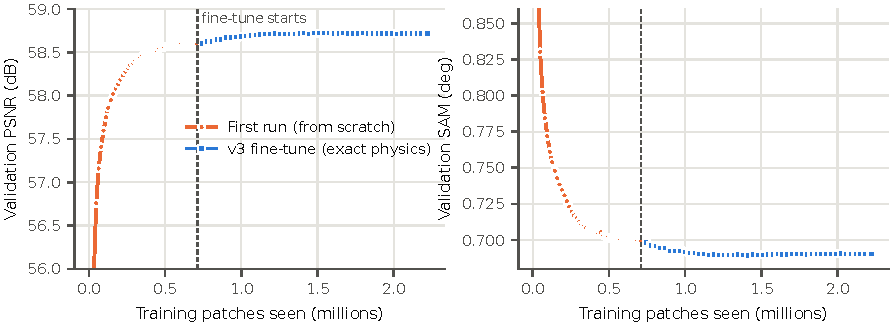
\includegraphics[width=\textwidth]{figures/training.pdf}
\caption{Chikusei: validation PSNR and SAM during training, plotted against the number of $64\times64$ training patches seen. The first run starts from random weights (its first two evaluations lie below the plotted range); v3 continues from its final weights with the exact border and the full loss.}
\label{fig:training}
\end{figure*}

\begin{figure*}[t]
\centering
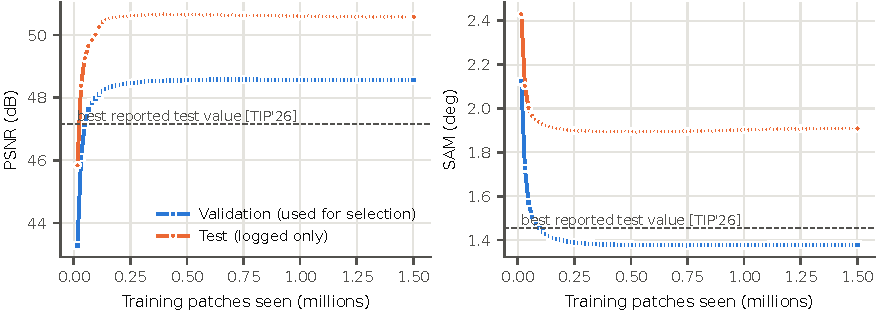
\includegraphics[width=\textwidth]{figures/training_pavia.pdf}
\caption{Pavia Centre: PSNR and SAM during training from scratch, on the validation patches (used to select the weights) and on the test images (logged only). The dashed line is the best value reported in~\cite{chen2026twostage} on the PSRT benchmark data.}
\label{fig:trainpavia}
\end{figure*}

\section{Robustness to Degradation Mismatch and Noise}
\label{sec:s-robust}
Published methods are usually trained and tested with the same degradation. We test the final models on inputs made with a different blur or a shifted spectral response, and with Gaussian noise added to both observations (Table~\ref{tab:robust}, Fig.~\ref{fig:robust}). Because the operators are explicit, PUFormer can also be given the true test-time operator without retraining (``swap''). On Chikusei, a blur mismatch costs 3.9--7.5~dB with the training operator. With the true blur swapped in, the loss is at most 0.26~dB for $\sigma$ between 1.5 and 3.0; with the zero-border operators of the first run, the same swap recovered only to 55.2--57.1~dB. A shifted spectral response is not compensated by the swap, which lowers the PSNR by a further 0.5~dB: the priors, trained with one response, rely on it beyond the data step. Noise is the main weakness of a model trained on noise-free data; PUFormer still exceeds GSA by 10.0~dB at 40~dB SNR and by 2.8~dB at 30~dB SNR. On Pavia Centre the blur behaves the same way: the training operator loses \pav{blur-fixed-loss-min}--\pav{blur-fixed-loss-max}~dB and the swapped-in true operator at most \pav{blur-swap-loss-max}~dB. Unlike on Chikusei, swapping in a shifted IKONOS response raises the PSNR slightly (by 0.2--0.3~dB), perhaps because an 8~nm shift is small relative to the 66--96~nm IKONOS bands, and the margins over GSA under noise are larger (\pav{noise40-margin}, \pav{noise35-margin} and \pav{noise30-margin}~dB at 40, 35 and 30~dB SNR).

% generated by make_tables.py - do not edit
\begin{table*}[t]
\centering
\caption{Robustness of the final models (test PSNR in dB / SAM in degrees). Fixed: training operator; swap: true operator supplied at test time; --: not applicable. The better PUFormer entry of each condition is in bold.}
\label{tab:robust}
\begin{tabular}{@{}lcccccc@{}}
\toprule
 & \multicolumn{3}{c}{Chikusei (PUFormer v3)} & \multicolumn{3}{c}{Pavia Centre (PUFormer)} \\
\cmidrule(lr){2-4}\cmidrule(l){5-7}
Condition & GSA & PUFormer fixed & PUFormer swap & GSA & PUFormer fixed & PUFormer swap \\
\midrule
Nominal & 43.20 / 2.73 & 58.15 / 0.72 & -- & 34.78 / 5.23 & 50.63 / 1.90 & -- \\
Blur $\sigma=1.5$ & 44.05 / 2.57 & 50.68 / 1.15 & \best{57.97 / 0.73} & 35.59 / 4.99 & 43.80 / 2.75 & \best{50.56 / 1.90} \\
Blur $\sigma=2.5$ & 42.77 / 2.82 & 54.26 / 0.88 & \best{58.05 / 0.72} & 34.36 / 5.36 & 47.30 / 2.14 & \best{50.59 / 1.90} \\
Blur $\sigma=3.0$ & 42.54 / 2.87 & 51.69 / 1.03 & \best{57.89 / 0.74} & 34.13 / 5.43 & 44.87 / 2.37 & \best{50.52 / 1.91} \\
SRF shift $-8$~nm & 42.86 / 2.91 & \best{53.01 / 1.20} & 52.54 / 1.31 & 34.58 / 5.36 & 49.46 / 1.99 & \best{49.75 / 2.03} \\
SRF shift $+8$~nm & 43.29 / 2.68 & \best{53.03 / 1.19} & 52.47 / 1.28 & 34.79 / 5.20 & 49.62 / 1.99 & \best{49.82 / 2.02} \\
Noise, 40~dB SNR & 43.04 / 2.85 & \best{53.03 / 1.39} & -- & 34.71 / 5.37 & \best{47.55 / 2.89} & -- \\
Noise, 35~dB SNR & 42.71 / 3.09 & \best{49.11 / 2.20} & -- & 34.57 / 5.64 & \best{44.36 / 4.19} & -- \\
Noise, 30~dB SNR & 41.84 / 3.67 & \best{44.62 / 3.69} & -- & 34.16 / 6.37 & \best{40.18 / 6.60} & -- \\
\bottomrule
\end{tabular}
\end{table*}


\begin{figure*}[t]
\centering
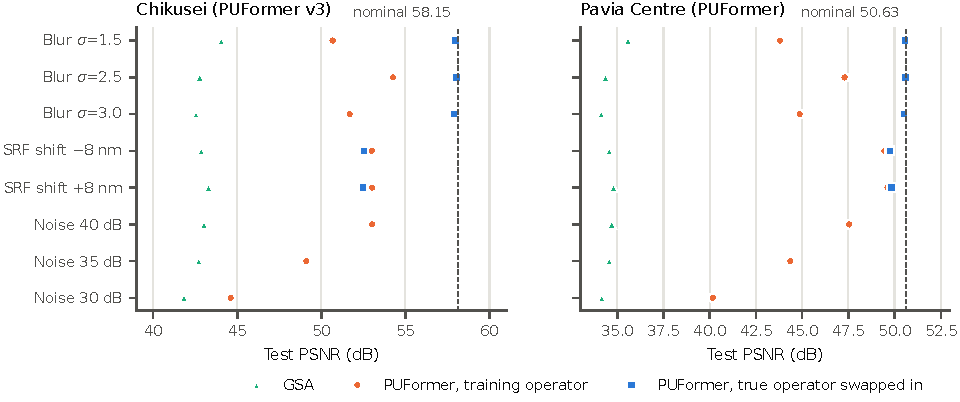
\includegraphics[width=\textwidth]{figures/robustness.pdf}
\caption{Test PSNR under degradation mismatch and noise on Chikusei (left) and Pavia Centre (right). The dashed line is the nominal PUFormer result.}
\label{fig:robust}
\end{figure*}

\section{Q2n on Chikusei}
\label{sec:s-q2n}
Q2n normalizes every band of every $32\times32$ block by the ground truth's own mean and standard deviation in that block, so an error that is small in absolute terms counts heavily in a band that is nearly flat within a block. Table~\ref{tab:q2n} and Fig.~\ref{fig:q2n} decompose the Q2n of the final model (\QtwonVthree). If the eight ultraviolet bands (363--404~nm) were reconstructed exactly, Q2n would rise to \QtwonExactUV; if the last 24 bands were exact as well, to \QtwonExactUVNIR. In the worst 10\% of blocks, the error energy of these eight bands equals \RelErrUV\ of the ground truth's local variance, against at most \RelErrMaxOther\ for any other group of eight bands. The fine detail of these bands cannot be predicted from the inputs: a least-squares injection of the multispectral detail, fitted on the test ground truth itself, reduces the band-1 error only from \OracleBicA\ to \OracleLinA~DN, while PUFormer reaches \OracleModelA~DN, and PUFormer is more accurate than this oracle in every band we checked.

Q2n is therefore nearly insensitive to overall accuracy on these test images: blending our reconstruction toward bicubic interpolation lowers the PSNR from \CalibPsnrHi\ to \CalibPsnrMid~dB but Q2n only from \CalibQHi\ to \CalibQMid\ (Fig.~\ref{fig:q2n}, right). The values reported in~\cite{chen2026twostage} do not follow PSNR in this way. Between 52.2 and 53.6~dB they range from 0.9832 (DCT) to 0.9963 (DDIF); of the 16 methods within the PSNR range of our curve, 11 lie above it and 5 below. U2Net, for example, is listed at 0.9928 at 50.55~dB, a value our implementation reaches only near 57.6~dB. We conclude that the Q2n values of~\cite{chen2026twostage} were most likely computed with a different implementation, normalization or test region, and that they are not directly comparable with ours.

\begin{table}[t]
\centering
\caption{Q2n analysis of PUFormer v3 (self-ensemble, test set)}
\label{tab:q2n}
\setlength{\tabcolsep}{4pt}
\begin{tabular}{@{}lc@{}}
\toprule
Setting & Q2n \\
\midrule
PUFormer v3 & \QtwonVthree \\
\quad bands 1--8 (363--404~nm) set to ground truth & \QtwonExactUV \\
\quad bands 1--8 and 105--128 set to ground truth & \QtwonExactUVNIR \\
\midrule
Deficit share, worst 10\% / 50\% of blocks & \DefTen\ / \DefFifty \\
\bottomrule
\end{tabular}
\end{table}

\begin{figure*}[t]
\centering
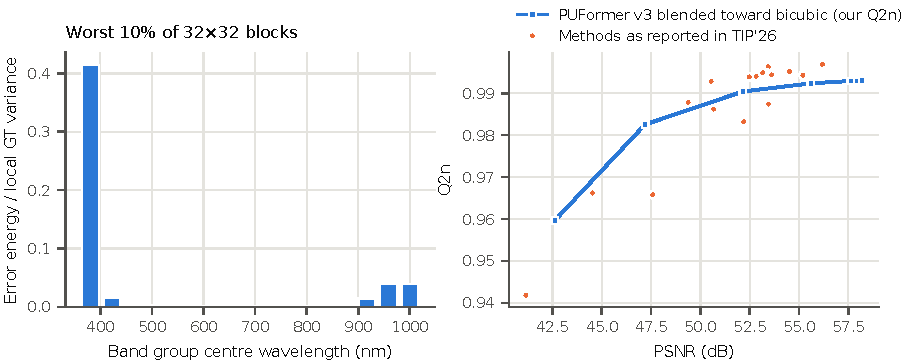
\includegraphics[width=\textwidth]{figures/q2n.pdf}
\caption{Left: error energy relative to the local ground-truth variance per group of eight bands in the worst 10\% of $32\times32$ blocks. Right: Q2n against PSNR when PUFormer's output is blended toward bicubic interpolation (our implementation), and the (PSNR, Q2n) pairs reported in~\cite{chen2026twostage}.}
\label{fig:q2n}
\end{figure*}

\section{SAM and Q2n on Pavia Centre}
\label{sec:s-pavia}
The Q2n shortfall on Pavia Centre comes from one test image, which also has the largest SAM (Table~\ref{tab:perimage}, Fig.~\ref{fig:sampavia}). On images 1, 3 and 4, Q2n is 0.9987--0.9991, at or above the best reported value, but SAM is still 1.55--1.68$^\circ$ (mean 1.60$^\circ$), above the best reported 1.454$^\circ$: the water image explains the Q2n gap, but only part of the SAM gap. Image 2 contains a stretch of the river Ticino: \pav{water-2}\% of its pixels have a positive normalized difference water index (green against near infrared), against \pav{water-1}, \pav{water-3} and \pav{water-4}\% in the other images, and its SAM is 2.72$^\circ$ and its Q2n 0.904. Water reflects little light, so its spectra are dominated by sensor noise that neither observation carries. The per-band noise that we estimate from the ground truth alone makes an angle of \pav{noise-floor-dark}$^\circ$ with the noise-free spectrum in the darkest tenth of the pixels, against \pav{noise-floor-bright}$^\circ$ in the brightest tenth. Over water PUFormer's SAM is \pav{sam-water}$^\circ$, over all other pixels \pav{sam-nowater}$^\circ$, and the darkest 10\% of the pixels account for \pav{sam-dark10}\% of its mean SAM. The same pixels make image 2 nearly flat within many $32\times32$ blocks, where Q2n divides the error by a very small local variance; image 2 alone carries 97\% of the Q2n deficit $\sum_i(1-\mathrm{Q2n}_i)$ of the four images.

\begin{figure*}[t]
\centering
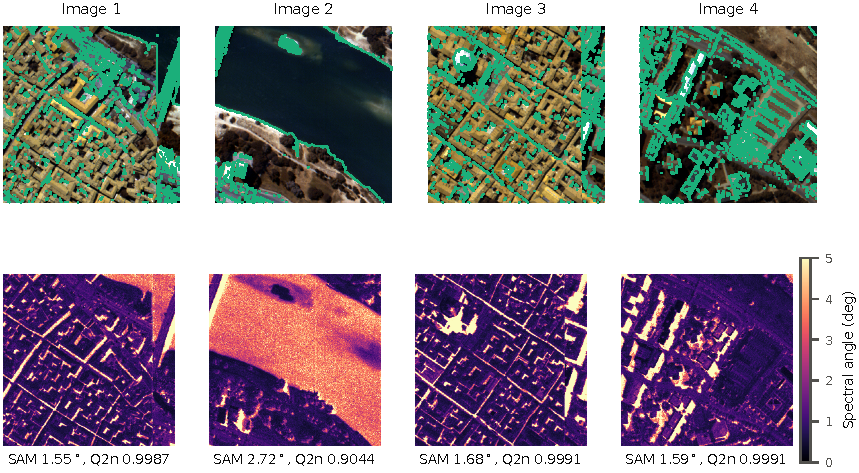
\includegraphics[width=\textwidth]{figures/sam_pavia.pdf}
\caption{The four Pavia Centre test images in false color (bands 57, 34 and 3; top), with water pixels (NDWI $>0$) outlined, and the spectral angle of PUFormer's reconstruction at every pixel (bottom; color scale clipped at 5$^\circ$).}
\label{fig:sampavia}
\end{figure*}

\section{Further Results of the Long-Trained Models}
\label{sec:s-more}
Table~\ref{tab:ours} lists the long-trained PUFormer models of the comparisons with reported results, together with bicubic interpolation and GSA, under every PSNR and SSIM definition in use, and Table~\ref{tab:perimage} gives the results of every test image. Chikusei images 5--8 are darker (their maximum is 0.36--0.47 of the dataset maximum), which lowers their strict SSIM but not their RMSE. Fig.~\ref{fig:visual} shows Chikusei image 7, the hardest test image, and Fig.~\ref{fig:visualpavia} Pavia Centre image \pav{visual-tile}, the hardest there. The errors of bicubic interpolation and GSA follow every field boundary and road (mean absolute errors of 164.7 and 64.8~DN), whereas both PUFormer models keep the error small and nearly uniform over the image (11.5 and 11.0~DN), apart from a few isolated pixels.

Fig.~\ref{fig:bandwise} shows the error of every band. PUFormer is more accurate than GSA in all 128 Chikusei bands, and the final model improves on the first run in every band, most at the red edge (700--760~nm), where the mean band RMSE falls from 7.9 to 4.2~DN (from 9.8 to 1.1~DN at 724~nm). The error is largest in the first eight bands (363--404~nm), which lie below the first WorldView-2 band and therefore receive no high-resolution detail from the multispectral image, and in the last bands near 1000~nm, where the sensor's signal-to-noise ratio drops.

% generated by make_tables.py - do not edit
\begin{table}[t]
\centering
\caption{The long-trained PUFormer models and the classical baselines under all PSNR and SSIM definitions. P$_\mathrm{g}$: peak = dataset maximum (headline); P$_\mathrm{i}$: peak = image maximum; P$_\mathrm{b}$: band-wise mean, peak 1. S$_1$: SSIM, data range 1; S$_\mathrm{i}$: data range = image maximum.}
\label{tab:ours}
\setlength{\tabcolsep}{3.2pt}
\resizebox{\columnwidth}{!}{%
\begin{tabular}{@{}lccccccc@{}}
\toprule
Method & P$_\mathrm{g}$ & P$_\mathrm{i}$ & P$_\mathrm{b}$ & S$_1$ & S$_\mathrm{i}$ & SAM & RMSE \\
\midrule
\multicolumn{8}{@{}l}{\textit{Chikusei}} \\
Bicubic & 33.63 & 28.20 & 35.25 & 0.8500 & 0.7404 & 4.406 & 321.8 \\
GSA~\cite{aiazzi2007gsa} & 43.20 & 37.76 & 44.82 & 0.9859 & 0.9778 & 2.730 & 107.7 \\
PUFormer, first run & 57.99 & 52.56 & 65.29 & 0.9989 & 0.9969 & 0.728 & 19.3 \\
PUFormer v3 & 58.15 & 52.71 & 66.26 & 0.9989 & 0.9969 & 0.717 & 19.1 \\
PUFormer v3, ensemble & 58.20 & 52.77 & 66.33 & 0.9989 & 0.9970 & 0.713 & 18.9 \\
\midrule
\multicolumn{8}{@{}l}{\textit{Pavia Centre}} \\
Bicubic & 25.52 & 25.11 & 25.87 & 0.6427 & 0.6282 & 6.555 & 436.3 \\
GSA~\cite{aiazzi2007gsa} & 34.78 & 34.37 & 35.19 & 0.9450 & 0.9438 & 5.229 & 157.9 \\
PUFormer & 50.63 & 50.22 & 51.11 & 0.9974 & 0.9970 & 1.895 & 23.7 \\
PUFormer, ensemble & 50.69 & 50.28 & 51.17 & 0.9974 & 0.9970 & 1.883 & 23.5 \\
\bottomrule
\end{tabular}}
\end{table}


% generated by make_tables.py - do not edit
\begin{table}[t]
\centering
\caption{Per-image results of the final models (self-ensemble)}
\label{tab:perimage}
\setlength{\tabcolsep}{3.4pt}
\begin{tabular}{@{}ccccccc@{}}
\toprule
Image & PSNR & S$_\mathrm{i}$ & S$_1$ & SAM & ERGAS & Q2n \\
\midrule
\multicolumn{7}{@{}l}{\textit{Chikusei, PUFormer v3}} \\
1 & 59.15 & 0.9994 & 0.9994 & 0.644 & 1.550 & 0.9957 \\
2 & 60.45 & 0.9985 & 0.9994 & 0.643 & 0.972 & 0.9967 \\
3 & 60.97 & 0.9987 & 0.9995 & 0.597 & 1.093 & 0.9962 \\
4 & 57.10 & 0.9981 & 0.9988 & 0.862 & 1.334 & 0.9917 \\
5 & 57.29 & 0.9951 & 0.9986 & 0.726 & 1.304 & 0.9929 \\
6 & 57.51 & 0.9957 & 0.9987 & 0.669 & 1.357 & 0.9913 \\
7 & 56.24 & 0.9953 & 0.9984 & 0.830 & 1.449 & 0.9913 \\
8 & 56.90 & 0.9947 & 0.9986 & 0.729 & 1.584 & 0.9889 \\
\cmidrule(l){1-7}
Mean & 58.20 & 0.9970 & 0.9989 & 0.713 & 1.330 & 0.9931 \\
\midrule
\multicolumn{7}{@{}l}{\textit{Pavia Centre, PUFormer}} \\
1 & 50.48 & 0.9977 & 0.9977 & 1.546 & 0.555 & 0.9987 \\
2 & 52.30 & 0.9949 & 0.9964 & 2.722 & 0.813 & 0.9044 \\
3 & 49.53 & 0.9979 & 0.9979 & 1.677 & 0.557 & 0.9991 \\
4 & 50.45 & 0.9975 & 0.9976 & 1.588 & 0.543 & 0.9991 \\
\cmidrule(l){1-7}
Mean & 50.69 & 0.9970 & 0.9974 & 1.883 & 0.617 & 0.9753 \\
\bottomrule
\end{tabular}
\end{table}


\begin{figure*}[t]
\centering
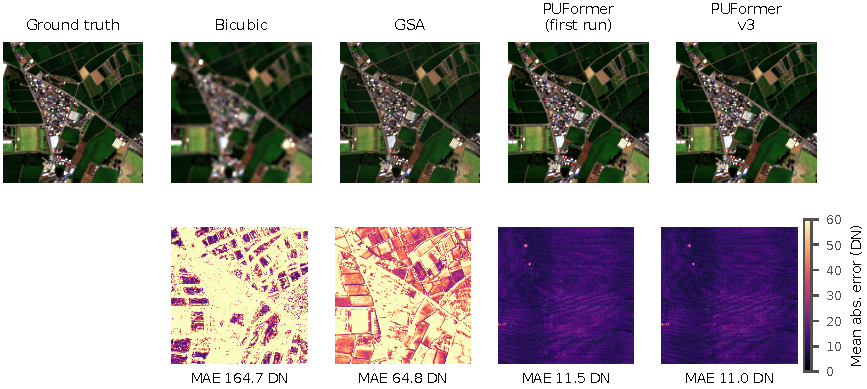
\includegraphics[width=\textwidth]{figures/visual.pdf}
\caption{Chikusei test image 7 in false color (bands 60, 40 and 20; top) and the mean absolute error over all bands in DN (bottom; color scale clipped at 60~DN).}
\label{fig:visual}
\end{figure*}

\begin{figure*}[t]
\centering
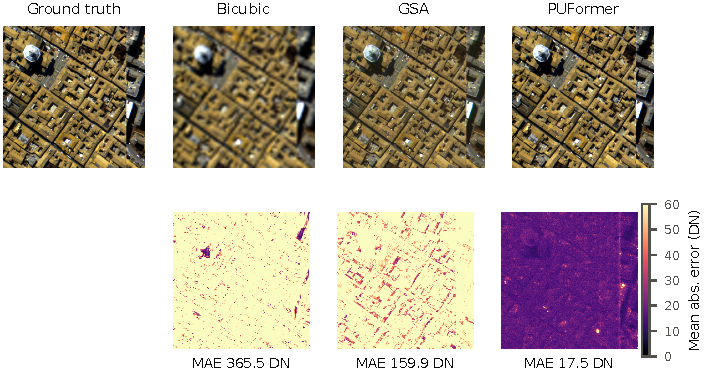
\includegraphics[width=0.8\textwidth]{figures/visual_pavia.pdf}
\caption{Pavia Centre test image \pav{visual-tile} in false color (bands 57, 34 and 3; top) and the mean absolute error over all bands in DN (bottom; color scale clipped at 60~DN).}
\label{fig:visualpavia}
\end{figure*}

\begin{figure*}[t]
\centering
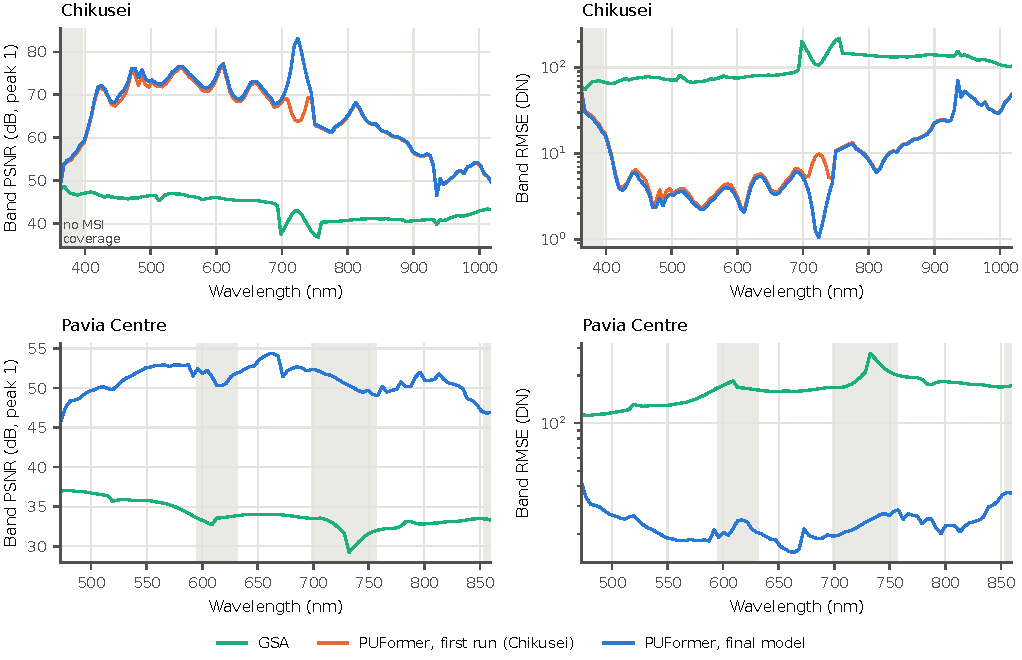
\includegraphics[width=\textwidth]{figures/bandwise.pdf}
\caption{Band-wise PSNR (left, peak 1) and RMSE in DN (right, log scale) over the test images of Chikusei (top) and Pavia Centre (bottom). Shaded ranges have no multispectral coverage: below the first WorldView-2 band for Chikusei, and between and beyond the IKONOS bands (50\% edges) for Pavia Centre.}
\label{fig:bandwise}
\end{figure*}

\section{Complete Benchmark Metrics}
\label{sec:s-full}
Table~\ref{tab:q1-full} lists all eight metrics of every method in the equal-budget benchmark; the per-job result files, including per-image values and training curves, are in the public repository.

\qtab{q1_full}

\bibliographystyle{IEEEtran}
\bibliography{references}

\end{document}
